\documentclass[12pt,letterpaper]{report}
%for roman numeral sectioning
\renewcommand{\thesection}{\Roman{section}} 
%\renewcommand{\thesubsection}{\thesection.\Roman{subsection}}


%Set depth of numbering
\setcounter{secnumdepth}{1} % only chapter and sections will be numbered
\setcounter{tocdepth}{2}    % entries down to \subsubsections in the TOC
%make 1 inch margins.

\usepackage[margin=1in]{geometry}

%page number top right (comment it all out if you want page num on bottom middle)
%\usepackage{fancyhdr}
%\pagestyle{fancy}
%\renewcommand{\headrulewidth}{0pt}
%\fancyhf{}
%\fancyhead[R]{\thepage}


%underline section titles
%\usepackage[explicit]{titlesec}
%\usepackage{ulem}
%
%\titleformat{\section}
%  {\normalfont\large\itshape}{\thesection}{1em}{\uline{#1}}
  
\usepackage[latin1]{inputenc}
\usepackage{amsmath}
\usepackage{amsfonts}
\usepackage{amssymb}
\usepackage{setspace}
%\usepackage{tocloft}
\usepackage[compact]{titlesec}
\usepackage[parfill]{parskip}

\usepackage{graphicx}
\usepackage{wrapfig}

\usepackage[super,comma]{natbib}

%To remove square brackets
\usepackage{ifthen}
\makeatletter
\renewcommand\@cite[2]{%
Ref.~#1\ifthenelse{\boolean{@tempswa}}
{, \nolinebreak[3] #2}{}
}
\renewcommand\@biblabel[1]{#1.}
\makeatother

%for quotes
\usepackage [english]{babel}
\usepackage [autostyle, english = american]{csquotes}
\MakeOuterQuote{"}

%This format looks alright.
\bibliographystyle{lastfirstabbrunsrtednat}

% Remove brackets from numbering in List of References
%\makeatletter
%\renewcommand{\@biblabel}[1]{\quad#1.}
%\makeatother

%Set the format of the titles
\titleformat{\chapter}[display]
{\singlespacing\bfseries\Huge}
{\titlerule\filright\Large\chaptertitlename\ \Large\thechapter}
{0pt}
{\filright}
[\titlerule]
\titlespacing*{\chapter}{0pt}{0pt}{*2}

\renewcommand{\thepage}{\roman{page}}% Roman numerals for page counter
\doublespacing

%Title page
\title{Comparative report of the Oxford Nanopore sequencing technology and current sequencers}
\author{Submitted to \\
Sister Hadden \\
for \\
English 316 \\
Brigham Young University \\
Provo, Utah \\
\today \\
\\
\\
by \\
Molly LoShiavo, Corianne Galloway, Kevin Boehme}
\date{}

%Change behavior of the contents
\makeatletter
\renewcommand*\@makechapterhead[1]{%
  %\vspace*{50\p@}%
  {\parindent \z@ \raggedright \normalfont
    \ifnum \c@secnumdepth >\m@ne
        \huge\bfseries \@chapapp\space \thechapter
        \par\nobreak
        \vskip 20\p@
    \fi
    \interlinepenalty\@M
    \centering \Huge \bfseries #1\par\nobreak
    \vskip 40\p@
  }}
\renewcommand*\@makeschapterhead[1]{%
  %\vspace*{50\p@}%
  {\parindent \z@ \raggedright
    \normalfont
    \interlinepenalty\@M
    \centering \Huge \bfseries  #1\par\nobreak
    \vskip 40\p@
  }}
  %This adds dots to the chapters
  \renewcommand*\l@chapter{\@dottedtocline{1}{0em}{1.5em}}
  \renewcommand*\l@subsection{\@dottedtocline{2}{5em}{3.2em}}
\makeatother

\begin{document}

%Title Page
\maketitle

\pagenumbering{gobble}
%Letter of Transmittal
%Just need to write it the old fashion way.
\begin{center}
\Huge\textbf{Technical Report}
\end{center}
\begin{flushleft}
\today \\[1\baselineskip]
\begin{singlespace}
English 316 \\
Sister Hadden \\
3004 JKB \\
Brigham Young University \\
Provo, UT 84602 \\
(801) 422-4704 \\[1\baselineskip]
\end{singlespace}
Dear Sister Hadden, \\[1\baselineskip]
As a group we are prepared to submit a copy of the Technical Report assignment for English 316 to our professor Sister Hadden.\\ [1\baselineskip]
The purpose of the report is to provide a comparison of current DNA sequencing technologies with the new Oxford nanopore technology. We focused on three of "next-generation" sequencing technologies to use for comparison: Illumina, Pacific Biosciences, and Ion Torrent. To compare these technologies we concentrated on three criteria to determine the best recommendation for the most efficient technology based on cost per megabase, time per run, and throughput per run. \\[1\baselineskip]
Please take time to look over our report. We are anxious for feedback so we can make the necessary improvements. If you have questions or comments please contact us at coric8@gmail.com, mollyloschiavo@gmail.com, or kevinlboehme@gmail.com. \\ [1\baselineskip]
Sincerely,\\[1\baselineskip]
Corianne Galloway, Molly LoSchiavo, Kevin Boehme
\end{flushleft}

\clearpage


%Table of Contents
%change level of indendation
%\setlength{\cftbeforetoctitleskip}{-2em}
%\cftsetindents{subsection}{.75in}{.75in}
\renewcommand*\contentsname{Table of Contents}
\setcounter{page}{3}
\renewcommand{\thepage}{\roman{page}}% Roman numerals for page counter
%\renewcommand{\cftpartleader}{\cftdotfill{\cftdotsep}} % for parts
%\renewcommand{\cftchapleader}{\cftdotfill{\cftdotsep}} % for chapters
\tableofcontents
\clearpage

%List of figures
%\thispagestyle{empty}

\addcontentsline{toc}{chapter}{\listfigurename}
\listoffigures
\clearpage

%List of Tables

\addcontentsline{toc}{chapter}{\listtablename}
\listoftables
\clearpage

%Abstract
%\addcontentsline{toc}{chapter}{Abstract}
%\begin{center}
%\Huge\textbf{Abstract}
%\end{center}
%\clearpage

%Start the report
\setcounter{page}{1}
\renewcommand{\thepage}{\arabic{page}}% Roman numerals for page counter

%Title
\begin{center}
\textbf{\Large{Comparative Report of the Oxford Nanopore sequencing technology and current sequencers}}
\end{center}

\section{Introduction}

The subject of our project is to evaluate the sequencing potential, cost, etc. of the up-and-coming Oxford nanopore technology as compared to the most popular next-generation DNA sequencing technologies.

As for the purpose of our study, we have provided a digestible and practical comparison of current sequencing technologies with that of the new Oxford nanopore technology. The results of this study will prove useful to a variety of groups. The largest branch of bioinformatics research deals with DNA sequencing pipelines and any potential "game-changing" technology will be of intense interest to all in this field. Health professionals could be interested in the results of this study if the results indicate a potential for rapid clinical applications i.e. by significantly reducing costs, or time for sequencing, etc. In addition, many business minded individuals, specifically in the biotech arena, follow sequencing technologies closely and the scope of this study should provide informative and perhaps tractable information to them.

The scope of this study involved the assessment of the new Oxford nanopore technology compared to the four most popular next-generation DNA sequencing technologies: Oxford Nanopore, Illumina, Ion Torrent, and Pacific Biosciences. To identify which of these technologies was most efficient, we focused on three main criteria: read length, cost per genome, and time per run.

The development of our project consisted of three steps: research, analysis, and solution. We first collected data and information regarding the various statistics and capabilities involved with the next-generation technologies. This information helped us formulate our background material as well as lay a foundation for analysis. This information was found on reputable websites such as www.AllSeq.com, www.biomedcentral.com, and www.illumina.com. We  also found data and information on the Oxford nanopore technology, as well as recent installments on its development and implementation. This information was found in reputable biotechnology journals such as Nature Biotechnology, Science, and Genome Research. We compared and analyzed our data according to our criteria mention in the scope of our project. After we completed our analysis, we formulated a recommendation for the most efficient sequencing technology.

\section{Background}

\subsection{Introduction to Sequencing}

DNA (deoxyribonucleic acid) is a molecule that is commonly referred to as "the blueprint of life". That is because the DNA found in just one of your trillions of cells contains all of the information needed to make, grow, and operate your body! This information is stored in the form of DNA sequence. DNA is composed of four kinds of molecules called nucleotides: adenine, guanine, cytosine, and thymine. For simplicity, these nucleotides are referred to as A, G, C, and T, respectively. DNA sequence is the order in which these nucleotides occur. This system may seem too simple to be responsible for creating and sustaining life, but that's the beauty of it; the system is incredibly simple and yet increasingly complex. Your DNA has a sequence that is 3 billion nucleotides long. In that sequence lies many of the answers to our questions about life and diseases such as cancer, Alzheimer's, autism, etc.

The firsts efforts to unearth this valuable sequence began in the 1970s. At this time, the prevailing sequencing technology (Sanger sequencing) was too primitive and too expensive to sequence anything larger than a couple hundred thousand nucleotides long. However, as new technologies emerged and public interest gained momentum over the following decades, the world of DNA sequencing experienced an event that changed it forever: The Human Genome Project. 

The mapping of the human genome was one of the largest collaborative projects in human history. With the presentation of this invaluable data to the public came a rush of new DNA sequencing technology. Many universities, research facilities, and private companies wanted to hitch a ride on the coattails of this new, exciting opportunity to perhaps get their own chance at changing the world. Through this, many brand-name technologies emerged such as Illumina, Ion Torrent, and PacBio. These technologies came to be known as "next-generation sequencing technologies" because of their technological advancement as compared to preliminary sequencing technologies like Sanger sequencing \cite{Shendure}. Still, as years have gone by, and as the field of genomics has grown, researchers yearn for faster, better sequencing technologies that can open up even more doors of opportunity. Specific goals that the field has set include reducing the cost of sequencing an individual's genome to less than \$1,000 and advancing medical and genomic research to someday realign the medical diagnostic framework so that patients will receive treatments specific to their genomic makeup \cite{Salto-Tellez}.

Oxford Nanopore is an up-and-coming sequencing technology that claims to be leading the world to a \$1,000 genome sequence with longer read length and shorter run time due to the fundamental design of the technology \cite{Maitra}. This fundamental design is what put Oxford Nanopore in the third-generation sequencing technologies category. We will now introduce each technology individually
	
\subsection{Illumina}

Nucleotides perform base-pairing between strands of DNA. In base-pairing, A and T only pair with each other, and C and G only pair with each other. Using this, Illumina employs "sequencing by synthesis" to sequence DNA. Sequencing by synthesis works by first isolating a single strand of DNA. Next, each of the four nucleotides is introduced to the strand. 
\begin{wrapfigure}{r}{0.5\textwidth}
\vspace{-20pt}
  \begin{center}
    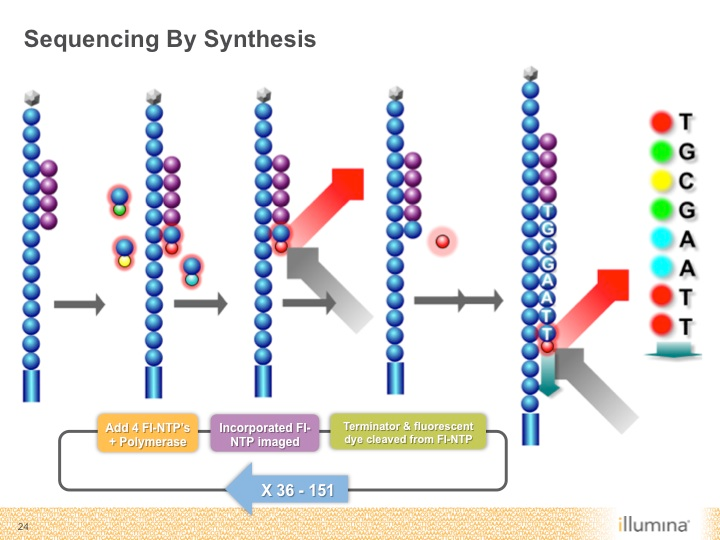
\includegraphics[width=0.48\textwidth]{illumina_fig.png}
  \end{center}
  \vspace{-20pt}
  \caption{Illumina}
  \vspace{-10pt}
  \label{fig:illumina}
\end{wrapfigure}
Because of base-pairing, only one of the nucleotides will attach to the first nucleotide on the strand. On the newly attached nucleotide is a fluorophore. Fluorophores fluoresce a specific color when activated by a laser. Each nucleotide is given a separate color. In Figure 1, T is red, G is green, C is yellow, and A is blue. After the nucleotide base-pairs to the DNA strand, the Illumina machine flashes a laser, and a camera records what color fluoresces. This tells the machine which nucleotide comes first. This process is then repeated until the entire DNA strand has been sequenced.

\subsection{Ion Torrent}

Ion Torrent's process for sequencing DNA, called "semiconductor sequencing", is fairly similar to that of Illumina, with some key differences. Both begin by isolating a single DNA strand. Rather than introducing all four nucleotides at the same time, Ion Torrent only introduces one base at a time. When a nucleotide base-pairs to the DNA strand, it releases a hydrogen ion. In the Ion Torrent machine, there is a hypersensitive pH meter. It can detect the single addition of a hydrogen ion in a solution. If, when the nucleotide is introduced to the DNA strand, the machine does not detect a change in pH, that nucleotide is removed, and the next kind is brought in. The process is repeated until the machine detects a change in pH. When that happens, the computer records which base was incorporated and starts over.
\clearpage
\subsection{PacBio}

\begin{wrapfigure}{r}{0.5\textwidth}
\vspace{-20pt}
  \begin{center}
    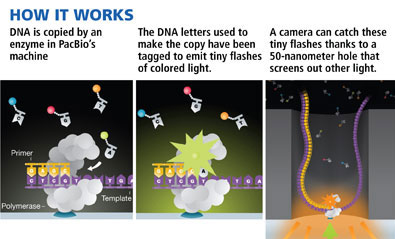
\includegraphics[width=0.48\textwidth]{pacbio_fig.png}
  \end{center}
  \vspace{-20pt}
  \caption{PacBio}
  \vspace{-10pt}
  \label{fig:pacbio}
\end{wrapfigure}

This technology is referred to as "single-molecule, real-time DNA sequencing" or "SMRT sequencing". Similar in concept to Illumina and Ion Torrent, but with its own important distinctions. SMRT sequencing begins by anchoring a single DNA polymerase molecule to the bottom of a tiny well. Next, a single DNA strand is introduced to the DNA polymerase. In addition, all four kinds of nucleotides are added to the solutions. These nucleotides have specifically colored fluorophores attached, as in Illumina. When DNA polymerase grabs the nucleotide that matches the DNA's sequence, it cleaves the fluorophore and activates it, emitting light (See Figure \ref{fig:pacbio}). A specialized camera recognizes the color of the light and records the respective base. The major advantage to this technology is DNA polymerase works extremely fast (around 1,000 base pairs per second) \cite{kelman}. We will discuss in our analysis why this trait is so advantageous.

\subsection{Oxford Nanopore}
\begin{wrapfigure}{r}{0.4\textwidth}
\vspace{-30pt}
  \begin{center}
    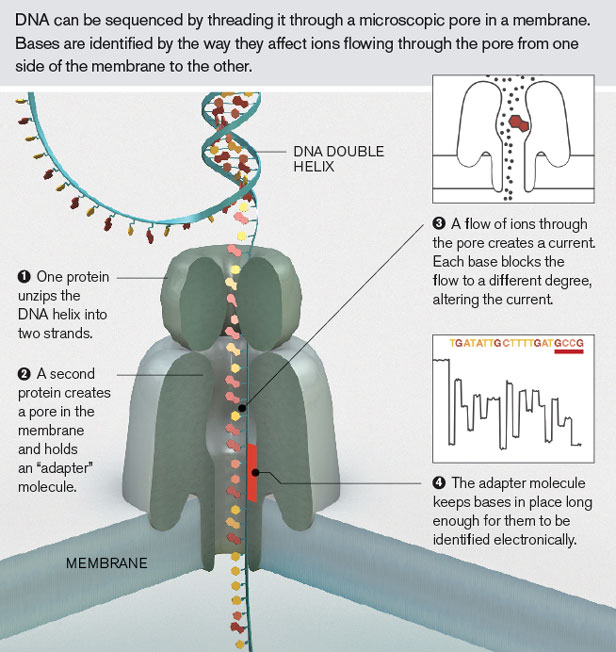
\includegraphics[scale=.35]{oxford_fig.png}
  \end{center}
  \vspace{-20pt}
  \caption{Oxford Nanopore}
  \vspace{-10pt}
  \label{fig:oxford}
\end{wrapfigure}

Oxford Nanopore utilizes "strand sequencing". The key to the workings of strand sequencing is a synthetically produced protein designed specifically for this task. This protein has a tube in the middle that is nanometers in diameter, making it small enough so only one strand of DNA can pass through at a time. This protein is also designed to fit into a tiny pore on a synthetic membrane. An electric current is then run through the membrane. Whenever anything passes through the small tube in the protein, it disrupts the current. Each molecule that passes through the protein creates its own distinct disruption. When a DNA strand, for example, is run through the protein, the disruptions made can be categorized into each of the four bases. In other words, the disruptions can be translated into the DNA's sequence (See Figure \ref{fig:oxford}) \cite{nanoporesite}. Ideally, because strand sequencing does not require any DNA synthesis, as do the other three technologies, it should be faster, more accurate, and cheaper. To determine if this is true, we selected three parameters to measure and compare each technology by. 

\section{Methodology}

\subsection{Cost per Megabase/Genome}

Considering the fact that the Human Genome Project cost around \$2.7 billion dollars, the cost of sequencing is a major limiting factor when considering projects \cite{Salto-Tellez}. Utilizing technologies that sequence at lower costs enable researchers to take on bigger projects and obtain more data \cite{Shendure}. Therefore, the cost it takes to obtain one megabase (1 million bases) of data is heavily considered by researchers when choosing what kind of sequencing technology to use.

Cost per megabase has been used for years as a standard price measurement for DNA sequencing technology. It is used by the National Human Genome Research Institute in their widely known and important benchmark graphs illustrating the decreasing costs associated with DNA sequencing 4. This measurement captures all of the direct 'production' costs of producing the raw sequencing data. These production costs include \cite{nhgriseqcosts}:

\begin{enumerate}
  \item Labor, administration, management, utilities, reagents, and consumables
  \item Sequencing instruments and other large equipment (amortized over three years)
  \item Informatics activities directly related to sequence production (e.g., laboratory information management systems and initial data processing)
  \item Shotgun library construction (required for preparing DNA to be sequenced)
  \item Submission of data to a public database
  \item Indirect Costs as they relate to the above items
\end{enumerate}

These are all important costs associated with producing DNA sequence data and should be captured in a cost per megabase measurement. However, many reports (often by the companies themselves) don't take all these costs into consideration and as a result price per final genome is sometimes a more accurate measure of sequencing costs.

Price per genome is an important measurement and is widely used. For instance, much hype has been made for the \$1,000 dollar genome and this is the goal set by the National Human Genome Research Institute. This information is usually supplied in addition to the price per megabase and both will be used in our report as price comparators.

The price of purchasing the actual sequencing machine is a critically important factor for those institutions looking to be able to sequence in-house. However, for others looking to outsource their DNA sequencing needs, this cost is not as important as the cost per megabase and cost per genome. So, for the scope of this report we will refrain from incorporating the cost of the actual machines into our comparison.

\subsection{Time per Run}
	
Time per run is an indicator of how quickly a technology can turn DNA template into sequence data. Next-generation technologies have really advanced with their applications paving the way for sequencing speed that is unprecedented \cite{Bao}. Researchers hold this quality of high importance because, as of now, genomic sequencing takes a considerable amount of time to complete. The Human Genome Project, for example, took about 13 years.4 Therefore, the shorter the run-time for assembly, the quicker each project can be completed. This is a crucial consideration not only for researchers, but also for investors who are anxious for good returns in a timely manner. A comparison between selected next-generation sequencing technologies in Van Dijk's research shows the importance of time per run in the technologies\cite{Maitra}. In the three technologies we focus on, we see that Illumina produces the most sets compared to Ion torrent and PacBio. Although time per run is of high importance, researchers also look at cost and error rates for the run \cite{van_Dijk}.
     
\subsection{Throughput per Run}
Throughput per run is a statistic that tells us how many base pairs are sequenced in a single run on a machine. It is important to consider throughput per run alongside with time per run because a machine with a short run-time is inefficient if it also produces a low throughput. In addition, a higher throughput per run increases efficiency in terms of cost. Each run of a machine costs a considerable amount of money, so the more throughput generated by each run, the more cost-efficient the machine. We used data from van Dijk, Loman, and Mikheyev for our analysis \cite{van_Dijk,Loman,Mikheyev}.

\subsection{Reservations}

\subsubsection{Validity of Machine Comparison}

Each technology discussed comes in many forms. For example, Illumina sells four different kinds of machines that use the same technology, but are built for different purposes (http://systems.illumina.com/systems/sequencing.html). We found that all but one of our chosen technologies offers a "desktop" machine, made to be efficient both in terms of money and time. However, these machines were not intended for use on large, data-intensive projects. Because the purpose of our report is to compare these technologies in terms of efficiency, we chose to use data collected from the desktop version of each technology. For Illumina, we used the MiSeq sequencer. For Ion Torrent, we used PGM, and for Oxford Nanopore, we used MinION.

One problem with this decision is that PacBio does not offer a desktop sequencer. They only offer one machine, the PacBio RS II, which is noted for its high accuracy and long reads, but not necessarily efficiency (http://www.pacificbiosciences.com/products/). While it would've been ideal to use data from a PacBio desktop unit, that was not possible, so we collected data for the RS II.

These circumstances reduce the validity of our comparison because the RS II was not built for the same purposes as the other three desktop sequencers. Despite this, we feel that given the situation, we have produced the best comparison possible to determine the most cost and time efficient technology.  

\subsubsection{Sources of MinIon data}

Since the Oxford nanopore technology is so new, there is significantly less data on its capabilities compared to the more established sequencers. The public's main source of unbiased data comes from a handful of published studies done by "early access" customers. The early access program allowed a small number of selected labs, institutions and individuals to purchase the nanopore sequencer in early spring 2014. These groups went on to do small sequencing projects using the MinIon usually sequencing small bacterial genomes. Besides giving a brief but useful explanation of the minION sequencer itself, these studies provide unbiased information on the data this machine produces and represent our main source of information regarding the price, speed, and accuracy of this technology.

\subsubsection{MinIon results vary by technology}

The results of a sequencing run vary by a lot of factors. Because MinIon is such a new technology many of its protocols and reagents are in flux. This is especially true of the critical flow cells that form the basic consumable reagent of the MinIon. Early access users were given a generation of flow cells called R6. Within a short time improvements were made and versions R7 (release in July 2014) and R7.3 (release in September 2014) were made available. 

\begin{table}
\vspace{-20pt}
\begin{center}
\begin{tabular}{lll}
\hline
 & R7 & R7.3 \\
\hline
Run Time & 72 hr & 48 hr \\
template reads & 43,656 (272Mb) & 39,819 (163 Mb) \\
complement reads & 23,338 (125 Mb) & 18,889 (84 Mb) \\
2D reads & 20,087 (131 Mb) & 11,823 (64.53 Mb) \\
Read Length (2D) & 6,543 & 5,458 \\
\hline
\end{tabular}
\caption{MinIon results of older R7 flow cell and R7.3.}
\end{center}
\label{table:summary_nanopore}
\end{table}

The advanced chemistry of these flow cells, while outside the scope of this report, plays a huge role in the quality of the results. This is demonstrated by certain studies which used older R6 concluded the technology is "close to useless"\cite{Mikheyev} while others using the R7 technology are able to produce improved results \cite{Quick}. A summary of the results of a recent study that implemented the two most recent iterations of the flow cell technology are shown in table \ref{table:summary_nanopore}.

\section{Data Summary}

\subsection{Cost Per Megabase/Genome}

\begin{wrapfigure}{r}{0.5\textwidth}
\vspace{-20pt}
  \begin{center}
    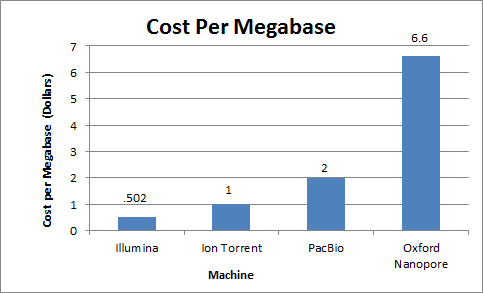
\includegraphics[width=0.48\textwidth]{cost_per_megabase.png}
  \end{center}
  \vspace{-20pt}
  \caption{Cost Per Megabase}
  \vspace{-10pt}
  \label{fig:cost_per_megabase}
\end{wrapfigure}

Figure \ref{fig:cost_per_megabase} displays our results for cost per megabase of sequenced data. The Oxford Nanopore cost was calculated using the reported flow cell price of \$1,000 and dividing it by the average throughput per run, which is 150 Mb. As evidenced from Figure 4, Oxford Nanopore produces the most expensive reads by a factor of at least 3 when compared to the other machines. Illumina had the cheapest cost per megabase at around 50 cents per million bases. This means that a human genome (3,000 Mb) could be sequenced for around \$1,500 whereas Oxford nanopore would cost \$19,800!


\subsection{Time Per Run}

\begin{wrapfigure}{r}{0.5\textwidth}
  \vspace{-20pt}
  \begin{center}
    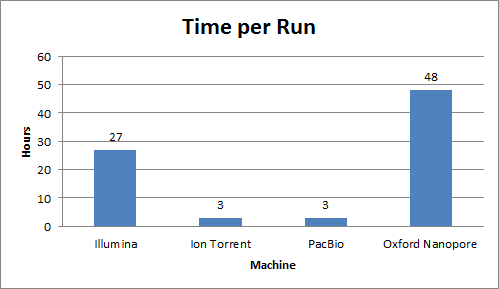
\includegraphics[width=0.48\textwidth]{time_per_run.png}
  \end{center}
  \vspace{-20pt}
  \caption{Time Per Run}
  \vspace{-10pt}
  \label{fig:time_per_run}
\end{wrapfigure}

In the three technologies we focus on, we see that Illumina produces the most sets compared to Ion torrent and PacBio. Although time per run is of high importance, researchers also look at cost and error rates for the run \cite{van_Dijk}. For example, in the Oxford nanopore technology, the MinION produced 20-30 percent error in the reads while the run time is about 48 hours \cite{karownotready}.

\subsection{Throughput per Run}

\begin{wrapfigure}{r}{0.5\textwidth}
\vspace{-20pt}
  \begin{center}
    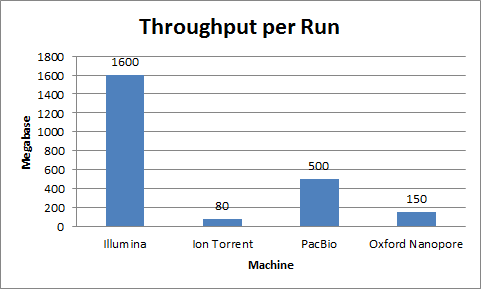
\includegraphics[width=0.48\textwidth]{throughput_per_run.png}
  \end{center}
  \vspace{-20pt}
  \caption{Cost Per Megabase}
  \vspace{-10pt}
  \label{fig:throughput_per_run}
\end{wrapfigure}

Current next-generation technologies output anywhere from 25 to 20,000 base pairs per read \cite{Shendure}. Table 2 is an example of a comparison of read lengths between next generation technologies \cite{van_Dijk}. Out of the five technologies listed in the graph, we focused on Illumina, Ion torrent, and PacBio. As seen in van Dijk's graph PacBio leads its competitors in read length with 20 kb making it ideal for finishing genome assemblies. Ion torrent and Illumina range between 300 and 400 length reads. Although PacBio produces the most reads, other factors i.e. cost and time per run need to be considered. Again, comparing the Oxford nanopore with the other technologies it was sub par as one of the runs was 24 hours and produced fewer than 25 reads; about 1 megabase of data \cite{karownotready}.  

\section{Discussion}

\begin{wrapfigure}{r}{0.5\textwidth}
\vspace{-20pt}
  \begin{center}
    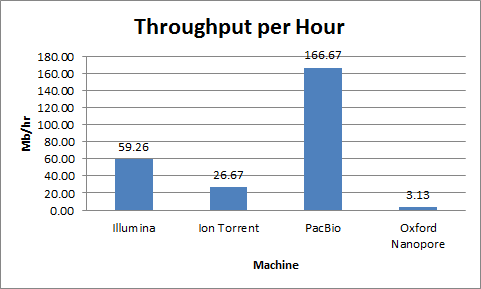
\includegraphics[width=0.48\textwidth]{throughput_per_hour.png}
  \end{center}
  \vspace{-20pt}
  \caption{Throughput Per Hour}
  \vspace{-10pt}
  \label{fig:throughput_per_hour}
\end{wrapfigure}

To interpret our results, we combined our data found for time per run and throughput per run to create a new measurement, throughput per hour, measured in megabases. We did this by multiplying the inverse of our time per run statistics by throughput per run. Figure \ref{fig:throughput_per_hour} shows our results. This interpretation suggests that PacBio is by far the most efficient in terms of time, producing 166.67 megabases of sequencing data per hour, and Oxford Nanopore is definitely the least efficient in terms of time, producing a mere 3.13 megabases of sequencing data per hour. 

Having determined the most efficient machine in terms of time, we will now discuss the machine that is the most efficient in terms of cost. Referring back to Figure \ref{fig:cost_per_megabase}, we see that Illumina is the most cost efficient, costing only .502 dollars to sequence one million bases, but Oxford Nanopore, once again, is the least efficient, costing \$6.60 to sequence on million bases. As mentioned before, this seemingly small price difference is very significant when sequencing billions of bases.

From this analysis, we have concluded that Illumina is more efficient in terms of cost, and PacBio is more efficient in terms of time. To determine which of the two is the most efficient all-around, we will compare the degrees to which each is the most efficient. From our data, we calculated ratios of each measurement and determined that Illumina is 3.98 times more cost-efficient than PacBio, whereas PacBio is only 2.81 times more time-efficient than Illumina

\section{Conclusion}
In this report, we aim to determine if Oxford Nanopore is more cost-efficient and time-efficient than the leading DNA sequencing technologies and if not, to determine which technology is the most efficient. To determine this, we gathered research on four technologies (Illumina, Ion Torrent, PacBio, and Oxford Nanopore). We compiled statistics of cost per megabase, time per run, and throughput per run. From these data, we combined time per run and throughput per run to generate a new measurement, throughput per hour. Throughput per hour indicated to us which machine was the most efficient in terms of time, and cost per megabase indicated to us which machine was the most efficient in terms of money.

From our analysis, we have determined that Oxford Nanopore is far from being more efficient than the other leading technologies. In fact, it is, by a large margin, the least efficient of those that we compared. Because of this result, we then determined which of the current technologies is the leader in efficiency.

We conclude that Illumina provides the most cost-efficient and time-efficient desktop machine (MiSeq). While PacBio was more efficient in terms of time, Illumina was more efficient in term of cost to such a higher degree, that we suggest that it beats out PacBio when considering both measures of efficiency.

As the field of genomics grows, many researchers and institutions around the world are considering investing in a DNA sequencing machine. This research can be of great value to those who are considering purchasing Oxford Nanopore's MinION unit because of all the public hype the machine is receiving. However, we find that they will save a lot more time and money if they instead invest in purchasing Illumina's MiSeq unit.

Thank you for reading our report. If there are any questions, comments, or clarifications, we can be contacted by email at any of these addresses: mollyloschiavo@gmail.com, kevinlboehme@gmail.com, coric8@gmail.com.


% The bibtex filename
\addcontentsline{toc}{chapter}{References}
\bibliography{references}
\clearpage

%Appendix
\addcontentsline{toc}{chapter}{Appendix}
\begin{center}
\Huge\textbf{Appendix}
\end{center}
\setcounter{section}{0}
\section{Glossary}

\textbf{DNA}: Deoxyribonucleic acid. A molecule whose sequence of nucleotides (see below) contains the information a cell needs to produce all proteins necessary for survival. Each cell in the human body contains a complete set of these "instructions". 

\textbf{Nucleotide}: A building block of DNA. Also known as a "base" or "base pair". There are four kinds: A, G, C, and T. The order of nucleotides determines the DNA's sequence.

\textbf{Genome}: The entire DNA sequence found in an organism's cell. Contains all the information for creating, growing, and sustaining that organism. The human genome is around 3 billion base pairs long. 

\textbf{Fluorophore}: Molecule that fluoresces a particular color when activated. Can be activated by a laser (as in Illumina) or by DNA polymerase (as in PacBio). In sequencing, particular colors of fluorophores are attached to particular bases. For example, all C's may be attached to red fluorophores, all T's may be attached to green fluorophores, all G's may be attached to blue fluorophores, and all A's may be attached to yellow fluorophores. 

\textbf{Base-pair}: A chemical bond between two nucleotides. A and T bond exclusively, and C and G bond exclusively. DNA is naturally found in a state where all of it's nucleotides are base-paired to the nucleotides of another DNA strand. This term is often interchangeable with "nucleotide" and "base". 

\textbf{Flow cells}: A consumable reagent for the Oxford Nanopore MinIon that contains all components necessary for one "sequencing run". Houses the chemistry and nanopores needed to sequence  and produce the sequence data.

\textbf{DNA polymerase}: Enzyme (protein) that dramatically increases the speed of the nucleotide base-pairing process by matching each base in a DNA strand with it's complementary base and creating the bond that holds the two bases together. 

\textbf{Megabase}: One million base-pairs. Used as a unit of measurement for how many bases were sequenced. 

\clearpage

\end{document}